\documentclass[../main.tex]{subfiles}

\begin{document}
\section{Physically Based Rendering}

\subsection{Wstęp}

Rozważania na temat modelu zgodnego z fizyką rozpoczniemy od zrozumienia w jaki
sposób wiązka światła zachowuje się po zderzeniu z idealnie równą powierzchnią.

Wiązka światła uderzająca w powierzchnię rozdziela się na dwie części, poprzez
dwa zjawiska: odbicie oraz refrakcję. Część energii wiązki światła w której
doszło do odbicia jest wysłana na zewnątrz obiektu bez wchodzenia w jego
materię. Część energii, która została uległa refrakcji wchodzi wgłąb obiektu,
gdzie zachodzą kolejne kolizje z materią, przez co znów dochodzi do powyższego
zjawiska, tym razem we wnętrzu obiektu. Część tego światła może wydostać się
z obiektu i dotrzeć do obserwatora. Zauważmy, że energia która dociera do
obserwatora musi być mniejsza lub równa energii wiązki światła - ta właściwość
jest jednym z filarów podejścia fizycznie poprawnego.

W modelach matematycznych zakładamy, że ponowne wyjście energii która była
poddana refrakcji następuje w tym samym punkcie, w którym promień zderzył się z
powierzchnią (rys. \ref{fig:ReflectionRefraction}).

Istnieją techniki które biorą pod uwagę możliwość ucieczki energii w innym
miejscu, ale skomplikowałyby one rozważania na których skupia się ta praca.
(Subsurface scattering, renderowanie skóry itd.)

% Rysunek odbicia z płaską powierzchnią (model uproszczony)
\begin{figure}[h]
  \centering
  \begin{tikzpicture}
    %\draw[help lines] (-5,-1) grid (5,5);
    \draw [thick] (-5.0,0.0) -- (5.0,0.0);

    % Specular
    \foreach \i in {0,...,5} {
      \pgfmathtruncatemacro{\angle}{90+30+(\i / 5) * 30};
      \draw [-Triangle, blue] (0,0) -- ( {3*cos(\angle)}, {3*sin(\angle)} );
    }

    % Diffuse
    \foreach \i in {1,...,15} {
      \pgfmathtruncatemacro{\angle}{(\i / 16) * 180};
      \draw [-Triangle, gray] (0,0) -- ( {2*cos(\angle)}, {2*sin(\angle)} );
    }

    \draw [fill] (2,2) circle [radius=0.05] node [above] {\Large\faLightbulbO};
    \draw  [-{Triangle[scale=2]}] (2,2) -- (0,0);
  \end{tikzpicture}
  \caption{Przybliżony model interakcji wiązki światła z powierzchnią}
  \label{fig:ReflectionRefraction}
\end{figure}

W naturze żaden materiał jest idealnym lustrem, w odpowiednio dużym
przybliżeniu zauważymy nierówności niedostrzegalne gołym okiem, a w odniesieniu
do grafiki komputerowej nierówności są dużo mniejsze od pojedynczego piksela
(rys. \ref{fig:Microstructure}).

\begin{figure}[h]
  \centering
  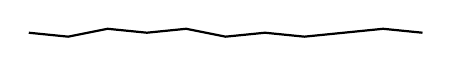
\begin{tikzpicture}
    \draw [thick]
      (0.0,0.15) --
      (0.5,0.10) --
      (1.0,0.20) --
      (1.5,0.15) --
      (2.0,0.20) --
      (2.5,0.10) --
      (3.0,0.15) --
      (3.5,0.10) --
      (4.0,0.15) --
      (4.5,0.20) --
      (5.0,0.15);
  \end{tikzpicture}
  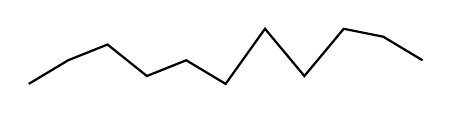
\begin{tikzpicture}
    \draw [thick]
      (0.0,0.1) --
      (0.5,0.4) --
      (1.0,0.6) --
      (1.5,0.2) --
      (2.0,0.4) --
      (2.5,0.1) --
      (3.0,0.8) --
      (3.5,0.2) --
      (4.0,0.8) --
      (4.5,0.7) --
      (5.0,0.4);
  \end{tikzpicture}
  \vspace{0.25cm}
  \caption{Mikrostruktura powierzchni o różnej chropowatości}
	\label{fig:Microstructure}
\end{figure}

Modele GTR (General Trowbridge-Reitz) i inne bazują na podejściu
mikropowierzchni z których każda zachowuje się jak powierzchnia idealna. Modele
te, szacują statystycznie jaka część promieni przybywająca z kierunku $w_i$
zostanie odbita w zadanym kierunku $w_o$. Funkcję tą, którą dalej będziemy
nazywać funkcją *BRDF* (ang. *bidirectional reflectance distribution
function*).

Całość odbitego światła w kierunku $w_o$ oznaczymy przez:

$$
L_0 = \int_{\Omega} {
    f_r(p, \omega_i, \omega_o)
    L_i(w_i)
    (n \cdot \omega_i)
    d \omega_i
}
$$

Powyższe równanie nazywamy równaniem renderingu (ang. *render equatiton*).

\subsection{Podstawowe pojęcia radiometryczne}

Rozpocznijmy od podstawowego budulca wiązki światła - fotonu. Energia fotonu
o długości fali $\lambda$ może zostać policzona ze wzoru

$$ Q = \frac{hc}{\lambda} $$

gdzie $h$ jest stałą Plancka a $c$ prędkością światła.

Strumień promieniowania (inaczej moc promieniowania, ang. *radiant flux*) to
całkowita ilość energii przechodząca przez określoną powierzchnię w czasie
jednostkowym. Powyższe pojęcie dotyczy wszystkich fal elektromagmetycznych,
zatem jest ono poprawne również dla światła. Jednostką strumienia
promieniowania jest Watt ($\text{W}$).

$$
\Phi = \lim_{\Delta t \rightarrow 0}{
    \frac{\Delta Q}{\Delta t}=\frac{dQ}{dt}
}
$$

Irradiancją nazywamy strumień promieniowania na jednostkę powierzchni.

$$
E(p) =
    \lim_{\Delta \rightarrow 0} {
        \frac{\Delta \Phi(p)}{\Delta A}
    } =
    \frac{d\Phi(p)}{dA}
$$

$$
\Phi = \int_{A} {
    E(p)
    dA
}
$$

W tym miejscu warto zauważyć, że jeżeli powierzchnia $A$ jest nachylona do
strumienia światła $\Phi$ pod pewnym kątem $\alpha$ to irradiancja zmienia się
proporcjonalnie do czynnika $\cos \alpha$. Wynika to z geometrii **!dodać
rysunek będący dowodem geometrycznym!**.

W przypadku jednorodnym irradiancję możemy zdefiniować jako średnią moc
promieniowania na pewnej skonczonej powierzchni $A$:

$$
E = \frac{\Phi}{A}
$$

Dla przykładu, policzmy irradiancję dla światła punktowego w punkcie $p$ na
sferze o promieniu $r$ o środku w tym właśnie punkcie $p$.

$$ E = \frac{\Phi}{4 \pi r^2} $$

Kątem planarnym obiektu geometrycznego $G$ z punktu $p$ nazywamy kąt wyznaczony
przez dwie półproste rozpoczynające się w punkcie $p$ wyznaczające minimalny
obszar zawierający obiekt $G$. Miarą kąta planarnego jest *radian* (rad).

% Rysunek kąta geometrycznego
\begin{figure}[ht]
  \centering
  \begin{tikzpicture}
    \coordinate (orig) at (0,0);
    \coordinate (left) at (1,3);
    \coordinate (right) at (5,2);
    \draw (2,1) -- (left) -- (2,4) -- (right) -- (2,1);
    \draw [dashed] (left)--(orig)--(right);
    \draw pic[draw=red, <->, "$\theta$", angle eccentricity=1.5] {angle = right--orig--left};
  \end{tikzpicture}
  \caption{Kąt planarny obiektu geometrycznego}
  \label{fig:PlanarAngle}
\end{figure}

Kąt bryłowy jest rozszerzeniem kąta planarnego do trzech wymiarów. Kątem
bryłowym $s$ nazywamy powiechnię rzutu trójwymiarowego obiektu geometrycznego
$G$ na sferę jednostkową o środku w punkcie $p$. Kąt bryłowy mierzony jest
w *steradianach* (sr). Kąt bryłowy całej sfery jednostkowej wynosi
  $4\pi \:{sr}$.

***(obrazek kąta bryłowego)***

Kolejną miarą energii jest *intensywność*. Intensywność jest miarą rozkładu
gęstości mocy światła na kierunkach cite p.~328 pbrt. Warto na wstępie
zauważyć, że intensywność ma sens tylko i wyłącznie dla teoretycznych świateł
punktowych ze względu na sposób pomiaru kąta. Wartość tą możemy zdefiniować w
następujący sposób:

$$
I = \lim_{\Delta\omega \rightarrow 0} {
    \frac{\Delta\Phi}{\Delta\omega}
} = \frac{d\Phi}{d\omega}
$$

$$
\Phi = \int_{\Omega} {I(\omega) d\omega}
$$

gdzie $\omega$ rozumiemy wektor określający kierunek ze środka jednostkowej
sfery do punktu leżącego na jej brzegu.

Dla przykładu intensywność jednorodnego światła punktowego wynosi:

$$
I = \frac{\Phi}{4\pi}
$$

Poprzez $E_{\omega}$ oznaczmy irradiancję powierzchni prostopadłej do kierunku
$\omega$. Radiancją $L$ nazywamy miarę irradiancji $E_{\omega}$ w odniesieniu
do kąta bryłowego:

$$
L(p, \omega) = \lim_{\Delta\omega \rightarrow 0} {
  \frac{\Delta E_{\omega} (p)}{\Delta\omega}
} =
\frac{d E(p)}{d \omega}
$$

Bardzo ważną obserwacją jest to, że radiancja nie jest mierzona względem
irradiancji powierzchni na której leży $p$, ma to na celu wyeliminowanie
czynnika $\cos \alpha$ z definicji cite:3, p.339. Jednstką radiancji jest "flux
density" na jednostkę powierzchni na jednostkę kąta bryłowego.

\subsection{Reflectance equation}

BRDF $f_r(p, \omega_o, \omega_i)$

- $\omega_i$ - kierunek przychodzący (od światła)
- $\omega_o$ - kierunek wychodzący (do oka)

*Light transport equation / Reflectance equation*:

$$
L_o(p, \omega_o) =
  L_e(p, \omega_o) +
  \int_{\mathbb{S}^2} {
    f(p, \omega_o, \omega_i)
    L_i(p, \omega_i)
    \cos \theta_i
    d\omega_i
  }
$$

- $f$ - BSDF
- $L_e$ - wyemitowana radiancja z punktu $p$ w kierunku $\omega_o$

$$
L_o(\omega_v) = \int_{\Omega} {
    f_r(\omega_l, \omega_v)
    L_i(\omega_l)
    (n \cdot l)
    d \omega_i
}
$$

Warunki PBR

1. Odwracalność (ang. reciprocity):
	$f_r(\omega_l, \omega_v) = f_r(\omega_v, \omega_l)$

2. Zachowanie energii

$$
\forall_{\omega_l}, \int_{\Omega} {
    f_r(\omega_l, \omega_v)
    (n \cdot \omega_v) d\omega_o
}
$$

\end{document}
